\section{Dataset e costruzione del workload}
\label{sec:dataset}

Lo scenario è stato costruito a partire dal dataset relativo ai sensori ambientali BME280. È stata considerata
la finestra temporale di gennaio 2025 e il dataset, di dimensione pari a circa
6.36 GB, è stato analizzato in modo incrementale per evitare il caricamento
completo in memoria.

Una prima fase di preprocessing ha permesso di verificare la qualità dei dati,
filtrare le osservazioni esterne alla finestra temporale e individuare i
sensori dotati di coordinate geografiche valide. Delle variabili disponibili,
le coordinate geografiche sono state utilizzate per la costruzione della
topologia, mentre temperatura, umidità e pressione sono state mantenute come
misure da riprodurre durante l'esecuzione. Le variabili relative all'altitudine
e alla pressione al livello del mare, completamente prive di valori, sono state
escluse.

Lo studio è stato limitato all'area europea. Per ogni sensore è stata
determinata una posizione rappresentativa e le coordinate geografiche
WGS84 sono state proiettate nel sistema metrico EPSG:3035, in modo da
applicare il clustering su distanze spaziali coerenti. La popolazione
risultante comprende 5102 sensori europei localizzabili.

La suddivisione in Edge Site è stata ottenuta tramite K-Means sulle coordinate
proiettate. Sono stati valutati valori di $k$ compresi tra 5 e 15 utilizzando
il Silhouette Score come criterio principale di selezione, affiancato
dall'inertia e dal raggio massimo dei cluster come indicatori diagnostici.
La configurazione selezionata è risultata $k=13$, con Silhouette Score pari
a circa 0.521; l'elbow method individua invece $k=9$, utilizzato solamente
come riferimento diagnostico.

\begin{figure}[H]
    \centering
    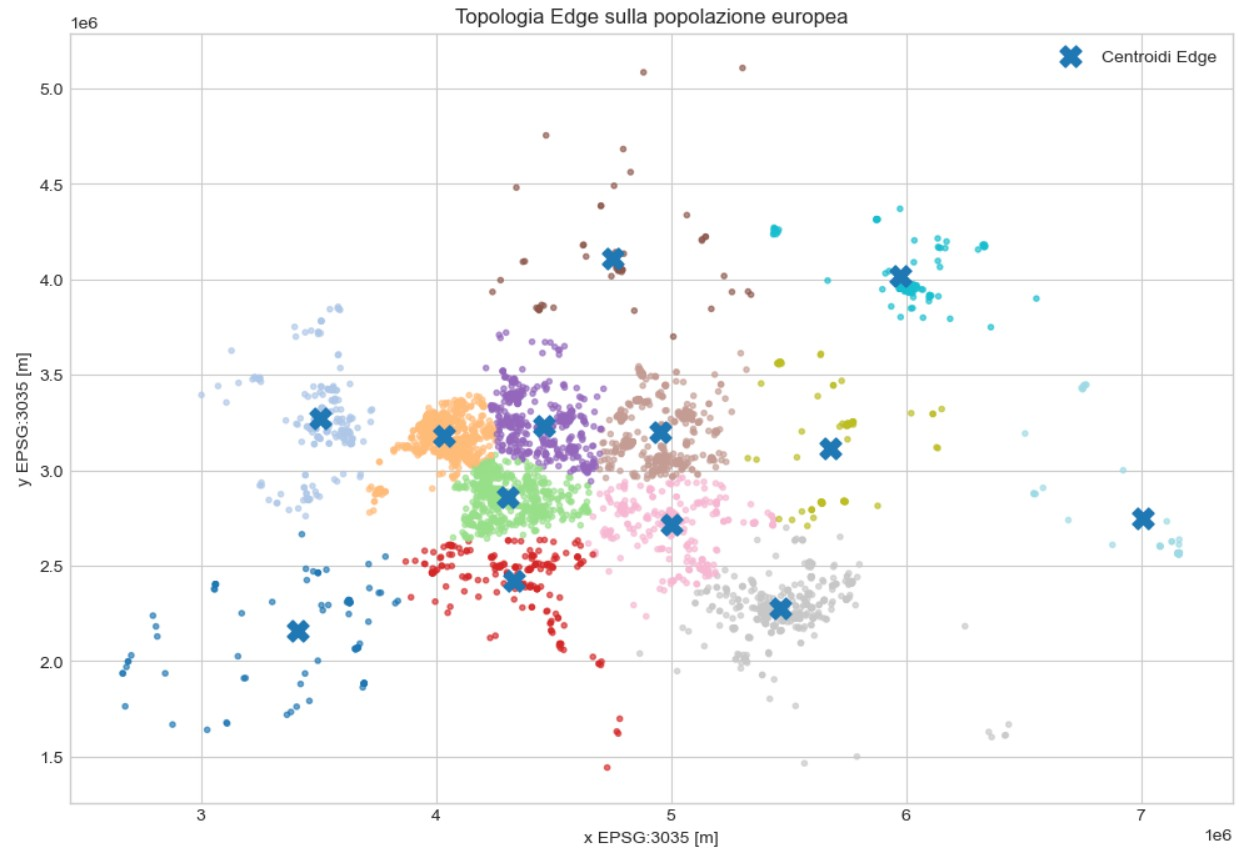
\includegraphics[width=\columnwidth]{figures/topologia_edge.jpg}
    \caption{Topologia geografica della popolazione europea e centroidi dei
    13 Edge Site.}
    \label{fig:edge-topology}
\end{figure}

Una volta determinata la topologia sull'intera popolazione europea, è stato
costruito il workload sperimentale selezionando 150 sensori. I sensori sono
stati distribuiti nel modo più uniforme possibile tra i 13 Edge Site
(11--12 sensori per Edge). La selezione all'interno di ciascun Edge è stata
effettuata utilizzando un seed pseudo-casuale fissato.
In questo modo ciascun Edge partecipa agli esperimenti con un numero
comparabile di sensori, pur mantenendo le differenze naturali nel tasso di
generazione degli eventi.

Infine, la fase di preprocessing produce due tipi di artefatti utilizzati
durante l'esecuzione: il file di topologia, che associa i sensori selezionati
agli Edge Site, e 13 shard di replay, uno per ciascun Edge, contenenti
identificativo del sensore, timestamp, pressione, temperatura e umidità.